% Final deck: 17 short slides in the order of the report (20:00 in total, 4:00 per member).
% Introduction, Model, Data and method, Results, Conclusion: the same sequence as report/main.tex.
% See ../notes/TEAM_PLAN.md section 2. Build with pdflatex from inside this folder (run it twice for the frame numbers).
% Each member's frames live in their own folder (M1/ ... M5/), one frame per slide, one presenter per slide.
% All numbers on the slides come from report/main.tex and results/.
\documentclass[aspectratio=169,10pt]{beamer}
% Shared look of the deck. Loaded by main_slides.tex and by every standalone preview (after \documentclass).
% Figures come from ../figs/ (main deck, compiled in slides/) or ../../figs/ (previews, compiled inside M1/ ... M5/).
\usepackage{graphicx,booktabs,amssymb,amsmath}
\usepackage{tikz}
\usetikzlibrary{arrows.meta,positioning}
\graphicspath{{../figs/}{../../figs/}}

\usetheme{default}
\setbeamertemplate{navigation symbols}{}
\definecolor{deckInk}{HTML}{1F2933}
\definecolor{deckAccent}{HTML}{1F4E79}
\definecolor{deckMuted}{HTML}{5F6B7A}
\definecolor{deckSoft}{HTML}{EAF1F8}
\definecolor{deckRule}{HTML}{9DB8D2}
\setbeamercolor{frametitle}{fg=deckInk}
\setbeamercolor{framesubtitle}{fg=deckInk!60}
\setbeamercolor{structure}{fg=deckAccent}
\setbeamerfont{frametitle}{series=\bfseries,size=\large}
\setbeamerfont{framesubtitle}{size=\scriptsize}
\setbeamertemplate{frametitle}{%
  \vspace*{4pt}\insertframetitle\par
  {\usebeamerfont{framesubtitle}\usebeamercolor[fg]{framesubtitle}\insertframesubtitle\par}
  \vskip3pt{\color{deckAccent}\hrule height 0.6pt}\vskip-4pt}
\setbeamertemplate{footline}{\hfill{\scriptsize\color{deckInk!50}\insertframenumber}\hspace*{10pt}\vspace*{6pt}}
\setbeamersize{text margin left=18pt,text margin right=18pt}

% one-sentence takeaway box used at the bottom of most slides
\providecommand{\pairTakeaway}[1]{%
  \par\vspace{3pt}\noindent
  \fcolorbox{deckRule}{deckSoft}{\parbox{\dimexpr\linewidth-2\fboxsep-2\fboxrule\relax}{\footnotesize\color{deckInk}#1}}}
\newcommand{\erfi}{\operatorname{erfi}}


\begin{document}

% Slide 1 | Introduction | M1 (Lakshya Satya) | 0:45 | cover, the idea and the roadmap
\begin{frame}[plain]
\centering\vspace{8pt}
{\color{deckInk}\Large\bfseries Pairs Trading with Mean-Reverting Stochastic Processes\par}
\vspace{2pt}
{\color{deckInk!75}\normalsize Ornstein--Uhlenbeck modelling, ADF-based cointegration selection\\and optimal trading bands\par}
\vspace{3pt}{\color{deckAccent}\hrule height 0.6pt}\vspace{5pt}
{\small\color{deckInk}Vismay Shanbhag \quad Tanishk Tasgaonkar \quad Lakshya Satya\\
Saatwik Tiwari \quad Nitin Sureshkumar\par}
\vspace{2pt}
{\footnotesize\color{deckMuted}MAC F244 \quad\textbullet\quad Semester I, 2026--27 \quad\textbullet\quad 15 November 2026\par}
\vspace{10pt}
{\normalsize\color{deckInk}Pairs trading bets that the price gap between two related stocks returns to its mean.\par}
\vspace{8pt}
\begin{columns}[T,onlytextwidth]
\column{0.31\textwidth}
\pairTakeaway{\textbf{1\ \ Detect}\\ Do the tests find real mean-reverting pairs?}
\column{0.31\textwidth}
\pairTakeaway{\textbf{2\ \ Model}\\ How well can the OU model be estimated?}
\column{0.31\textwidth}
\pairTakeaway{\textbf{3\ \ Trade}\\ Does any rule beat a simple one after costs?}
\end{columns}
\end{frame}
                  % 1  Introduction        M1  0:45
% Slide 2 | Model | M3 (Tanishk Tasgaonkar) | 2:15 | spread, OU process, exact discretisation
\begin{frame}{The spread follows an Ornstein--Uhlenbeck process}
\framesubtitle{Slide 2 \textbullet\ Model \textbullet\ M3 \textbullet\ 2:15}
\vspace{-2pt}
\begin{columns}[T,onlytextwidth]
\column{0.50\textwidth}
  \footnotesize\raggedright
  \textbf{\color{deckAccent}Model}
  {\scriptsize\[ X_t=\ln P^A_t-\beta\ln P^B_t-\mu \]}
  \[ dX_t=\kappa(\theta-X_t)\,dt+\sigma\,dW_t \]
  {\scriptsize\[ X_t=\theta+(X_0-\theta)e^{-\kappa t}+\sigma\!\int_0^t e^{-\kappa(t-s)}dW_s \]}
  \begin{itemize}\setlength{\itemsep}{1pt}
    \item $\kappa$ speed, $\theta$ level, $\sigma$ noise
    \item stationary law $N(\theta,\sigma^2/2\kappa)$; the gap halves in $\ln 2/\kappa$
  \end{itemize}
\column{0.46\textwidth}
  \footnotesize\raggedright
  \textbf{\color{deckAccent}Exact one-day step}\quad {\scriptsize ($\Delta=1/252$)}
  {\scriptsize\[ X_{t+\Delta}=a+bX_t+\varepsilon_t,\quad b=e^{-\kappa\Delta} \]}
  \begin{itemize}\setlength{\itemsep}{1pt}
    \item an AR(1): \textbf{OLS is maximum likelihood}
  \end{itemize}
  {\scriptsize\[ \hat\kappa=-\frac{\ln\hat b}{\Delta},\quad \hat\theta=\frac{\hat a}{1-\hat b},\quad \sigma_{eq}=\frac{\hat s_\varepsilon}{\sqrt{1-\hat b^2}} \]}
\end{columns}
\pairTakeaway{The step is exact, so a regression of tomorrow's spread on today's gives the speed, the level and the noise.}
\end{frame}
               % 2  Model               M3  2:15
% Slide 3 | Model | M4 (Vismay Shanbhag) | 1:00 | the ADF test
\begin{frame}{The ADF test asks whether $\kappa=0$}
\framesubtitle{Slide 3 \textbullet\ Model \textbullet\ M4 \textbullet\ 1:00}
\vspace{-2pt}
\begin{columns}[T,onlytextwidth]
\column{0.54\textwidth}
  \normalsize\raggedright
  \textbf{\color{deckAccent}The regression}
  {\small\[ \Delta X_t=a+\gamma X_{t-1}+\sum_{i=1}^{p}\delta_i\,\Delta X_{t-i}+\varepsilon_t \]
  \[ \gamma=e^{-\kappa\Delta}-1 \]}
\column{0.42\textwidth}
  \normalsize\raggedright
  \begin{itemize}\setlength{\itemsep}{2pt}
    \item $H_0:\gamma=0$ is $H_0:\kappa=0$, a random walk
    \item lagged differences clean the noise; lags chosen by AIC
    \item 5\% critical value $-2.86$, not $-1.65$
  \end{itemize}
\end{columns}
\pairTakeaway{How often the test succeeds depends on $\kappa T$, the number of half-lives in the window (E2a).}
\end{frame}
                    % 3  Model               M4  1:00
% Slide 4 | Model | M2 (Nitin Sureshkumar) | 1:00 | Engle--Granger cointegration
\begin{frame}{Engle--Granger: testing a pair in two steps}
\framesubtitle{Slide 4 \textbullet\ Model \textbullet\ M2 \textbullet\ 1:00}
\vspace{-2pt}
\large\raggedright
\begin{enumerate}\setlength{\itemsep}{3pt}
  \item regress $a_t=\mu+\beta b_t+u_t$ on the formation year: the residual $\hat u_t$ is the spread
  \item run the ADF test on $\hat u_t$, with a stricter critical value: about $-3.34$, instead of $-2.86$
  \item keep the pair only if it passes in \textbf{both directions} ($a$ on $b$ and $b$ on $a$)
\end{enumerate}
\pairTakeaway{Fitting $\beta$ makes unrelated prices look cointegrated (a spurious regression), so the threshold must be stricter.}
\end{frame}
          % 4  Model               M2  1:00
% Slide 5 | Model | M4 (Vismay Shanbhag) | 1:00 | the four trading rules
\begin{frame}{Four trading rules}
\framesubtitle{Slide 5 \textbullet\ Model \textbullet\ M4 \textbullet\ 1:00}
\vspace{-2pt}
\small\setlength{\tabcolsep}{4pt}
\begin{tabular}{@{}l@{\ \ }p{3.5cm}p{4.9cm}p{4.2cm}@{}}
  \toprule
  & Rule & Open when & Close when \\
  \midrule
  S0 & Distance (Gatev et al.) & gap of normalised prices $>2\sigma$ & the prices cross \\
  S1 & z-score (Chan) & $|z|>2$ & $|z|<0.5$ \\
  S2 & s-score (Avellaneda \& Lee) & $s<-1.25$ long, $s>1.25$ short & $s>-0.50$ long, $s<0.75$ short \\
  S3 & Optimal bands (Bertram) & $|s|\ge m^*$ & the opposite band \\
  \bottomrule
\end{tabular}\\[5pt]
{\footnotesize $z=X/\sigma_X$ and $s=(X-\hat\theta)/\sigma_{eq}$, where $X$ is the Engle--Granger spread}
\pairTakeaway{Thresholds are fixed in advance and never tuned on our results.}
\end{frame}
          % 5  Model               M4  1:00
% Slide 6 | Model | M5 (Saatwik Tiwari) | 1:15 | Bertram's optimal bands
\begin{frame}{Bertram's optimal trading bands (S3)}
\framesubtitle{Slide 6 \textbullet\ Model \textbullet\ M5 \textbullet\ 1:15}
\vspace{-2pt}
\normalsize\raggedright
One trade is a cycle: enter at $a$, exit at $m>a$, pay the round-trip cost $c$. First-passage times (backward equation $\tfrac12\sigma^2u''-\kappa x\,u'=-1$) give
{\normalsize\[ \mathbb{E}[T]=\frac{\pi}{\kappa}\Big[\erfi\!\Big(\frac{m\sqrt\kappa}{\sigma}\Big)-\erfi\!\Big(\frac{a\sqrt\kappa}{\sigma}\Big)\Big],\qquad
\mu(a,m)=\frac{m-a-c}{\mathbb{E}[T]} \]}
\begin{itemize}\setlength{\itemsep}{2pt}
  \item symmetric bands $a=-m$: maximise the return per unit time $\mu$ over $m$
\end{itemize}
\pairTakeaway{A higher trading cost pushes the best band $m^*$ outwards.}
\end{frame}
                % 6  Model               M5  1:15
% Slide 7 | Data and methodology | M2 (Nitin Sureshkumar) | 0:45 | the data
\begin{frame}{The data}
\framesubtitle{Slide 7 \textbullet\ Data and method \textbullet\ M2 \textbullet\ 0:45}
\vspace{-2pt}
\begin{columns}[T,onlytextwidth]
\column{0.50\textwidth}
  \footnotesize\setlength{\tabcolsep}{5pt}
  \begin{tabular}{@{}lll@{}}
    \toprule
    & US & India (NSE) \\
    \midrule
    Stocks   & 56 large caps & 26 \\
    Sectors  & 7 & 5 \\
    Period   & 2010--2026 & 2012--2026 \\
    Pairs per window & 196 & 55 \\
    \bottomrule
  \end{tabular}
\column{0.46\textwidth}
  \normalsize\raggedright
  \begin{itemize}\setlength{\itemsep}{2pt}
    \item daily adjusted closes from Yahoo Finance
    \item pairs only within a sector
  \end{itemize}
\end{columns}
\pairTakeaway{Today's large caps give the sample survivorship bias.}
\end{frame}
                   % 7  Data and method     M2  0:45
% Slide 8 | Data and methodology | M1 (Lakshya Satya) | 1:15 | walk-forward protocol and no look-ahead
\begin{frame}{Walk-forward protocol, no look-ahead}
\framesubtitle{Slide 8 \textbullet\ Data and method \textbullet\ M1 \textbullet\ 1:15}
\vspace{-2pt}
\centering
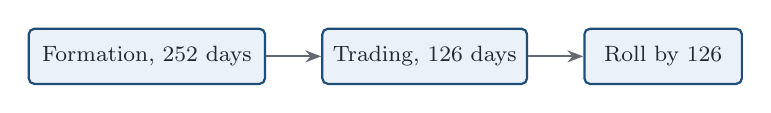
\begin{tikzpicture}[
    box/.style={rectangle, draw=deckAccent, fill=deckSoft, thick, rounded corners=2pt,
                minimum height=0.7cm, font=\footnotesize, text=deckInk},
    arr/.style={-{Stealth[length=2mm]}, thick, draw=deckInk!70}]
  \node[box, minimum width=3.0cm] (F) {Formation, 252 days};
  \node[box, minimum width=2.6cm, right=0.7cm of F] (T) {Trading, 126 days};
  \node[box, minimum width=2.0cm, right=0.7cm of T] (R) {Roll by 126};
  \draw[arr] (F) -- (T); \draw[arr] (T) -- (R);
\end{tikzpicture}\\[6pt]
\normalsize\raggedright
\begin{itemize}\setlength{\itemsep}{2pt}
  \item pairs and parameters come from the formation year only and stay frozen
  \item a signal at the close of day $t$ is traded at the close of $t+1$
  \item costs: 10 bp (US) or 15 bp (India) per stock, per trade
\end{itemize}
\pairTakeaway{Letting the parameters peek at the trading window would raise the s-score Sharpe ratio from about 0 to \textbf{3.6}.}
\end{frame}
               % 8  Data and method     M1  1:15
% Slide 9 | Results | M3 (Tanishk Tasgaonkar) | 1:45 | E1: how accurately can kappa be estimated?
\begin{frame}{E1: estimating the speed $\kappa$ is biased}
\framesubtitle{Slide 9 \textbullet\ Results \textbullet\ M3 \textbullet\ 1:45}
\vspace{-2pt}
\begin{columns}[T,onlytextwidth]
\column{0.52\textwidth}
  \centering
  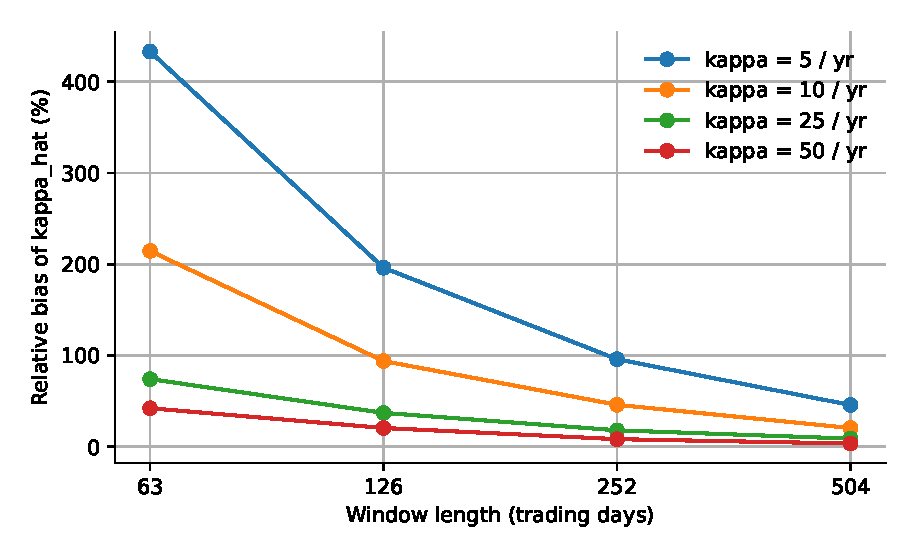
\includegraphics[width=\linewidth]{fig_e1_ou_estimation}
\column{0.44\textwidth}
  \footnotesize\raggedright
  \begin{itemize}\setlength{\itemsep}{3pt}
    \item one year of data: $\hat\kappa$ too high by \textbf{18\%} (7-day half-life) and \textbf{96\%} (35-day)
    \item the error halves each time the window doubles
  \end{itemize}
\end{columns}
\pairTakeaway{Pairs look faster, and more attractive, than they really are.}
\end{frame}
       % 9  Results E1          M3  1:45
% Slide 10 | Results | M4 (Vismay Shanbhag) | 0:45 | E2a: what can ADF detect?
\begin{frame}{E2a: one year sees only fast pairs}
\framesubtitle{Slide 10 \textbullet\ Results \textbullet\ M4 \textbullet\ 0:45}
\vspace{-2pt}
\begin{columns}[T,onlytextwidth]
\column{0.44\textwidth}
  \centering
  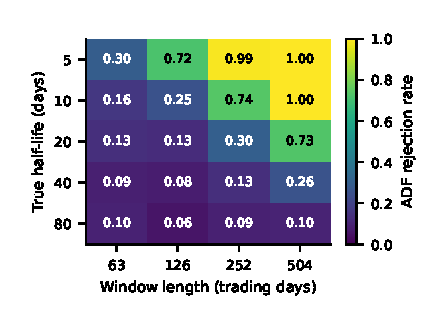
\includegraphics[width=\linewidth]{fig_e2_adf_power_report}
\column{0.52\textwidth}
  \footnotesize\raggedright
  How often ADF finds a gap that really closes, with one year of data:
  \begin{itemize}\setlength{\itemsep}{2pt}
    \item 5-day half-life: \textbf{99\%}
    \item 10 days: \textbf{74\%}
    \item 20 days: \textbf{30\%}
  \end{itemize}
\end{columns}
\pairTakeaway{Every pair we select has a half-life of 15 days or less.}
\end{frame}
              % 10 Results E2a         M4  0:45
% Slide 11 | Results | M2 (Nitin Sureshkumar) | 1:00 | E2b: size of the residual test
\begin{frame}{E2b: plain ADF finds false pairs}
\framesubtitle{Slide 11 \textbullet\ Results \textbullet\ M2 \textbullet\ 1:00}
\vspace{-2pt}
\begin{columns}[T,onlytextwidth]
\column{0.48\textwidth}
  \small\raggedright
  1{,}000 pairs of unrelated random walks, which are never cointegrated: how often is a pair wrongly found?\\[6pt]
  \footnotesize\setlength{\tabcolsep}{6pt}
  \begin{tabular}{@{}lr@{}}
    \toprule
    Critical values & Wrongly found \\
    \midrule
    Plain ADF & \textbf{16.9\%} \\
    Engle--Granger & \textbf{6.2\%} \\
    \midrule
    Intended level & 5\% \\
    \bottomrule
  \end{tabular}
\column{0.48\textwidth}
  \normalsize\raggedright
  \begin{itemize}\setlength{\itemsep}{2pt}
    \item plain ADF calls one unrelated pair in six cointegrated
    \item Engle--Granger is close to the intended 5\%
  \end{itemize}
\end{columns}
\pairTakeaway{The selection test must be stricter than plain ADF.}
\end{frame}
               % 11 Results E2b         M2  1:00
% Slide 12 | Results | M5 (Saatwik Tiwari) | 1:15 | E3: is Bertram's formula right?
\begin{frame}{E3: the formula is right, daily checking is slower}
\framesubtitle{Slide 12 \textbullet\ Results \textbullet\ M5 \textbullet\ 1:15}
\vspace{-2pt}
\begin{columns}[T,onlytextwidth]
\column{0.50\textwidth}
  \centering
  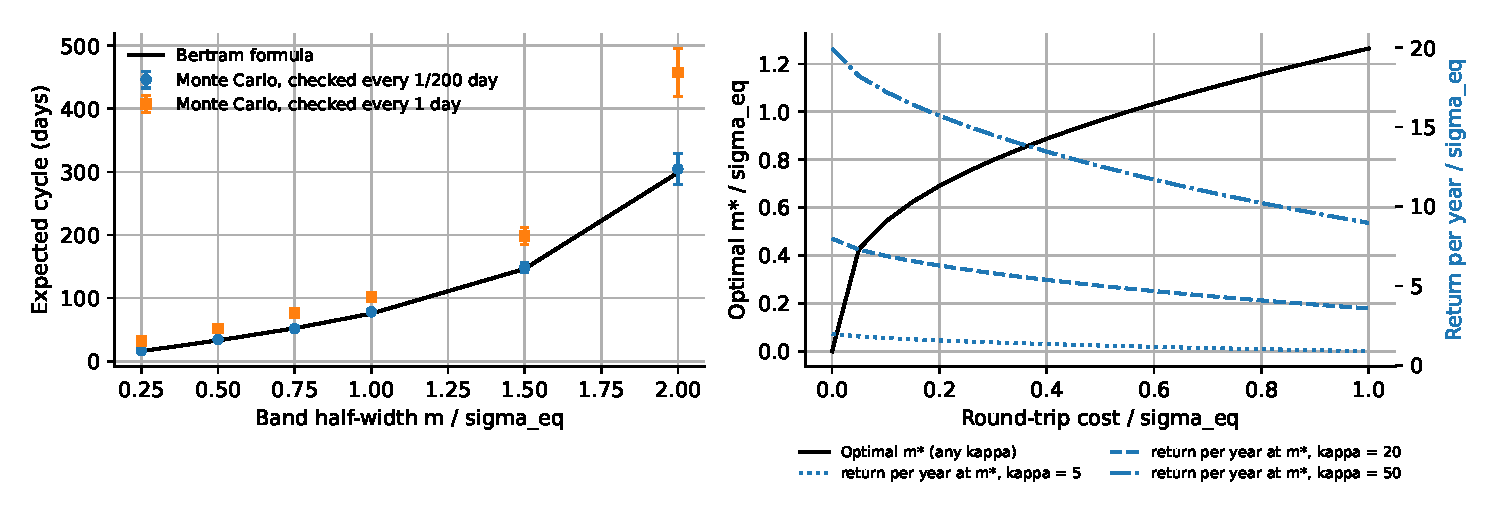
\includegraphics[width=\linewidth,trim=0bp 0bp 374bp 0bp,clip]{fig_e3_bertram}\\[1pt]
  {\scriptsize expected cycle time: formula against simulation}
\column{0.46\textwidth}
  \footnotesize\raggedright
  \begin{itemize}\setlength{\itemsep}{3pt}
    \item the formula is \textbf{exact}: it matches a numerical integration to $10^{-8}$
    \item checking prices once a day makes a cycle \textbf{35--99\% longer}
  \end{itemize}
\end{columns}
\pairTakeaway{The spread can cross a band and return between two daily looks.}
\end{frame}
          % 12 Results E3          M5  1:15
% Slide 13 | Results | M1 (Lakshya Satya) | 1:15 | E4, the perfect pair
\begin{frame}{E4: a perfect pair earns only about half its theory}
\framesubtitle{Slide 13 \textbullet\ Results \textbullet\ M1 \textbullet\ 1:15}
\vspace{-2pt}
\begin{columns}[T,onlytextwidth]
\column{0.58\textwidth}
  \centering
  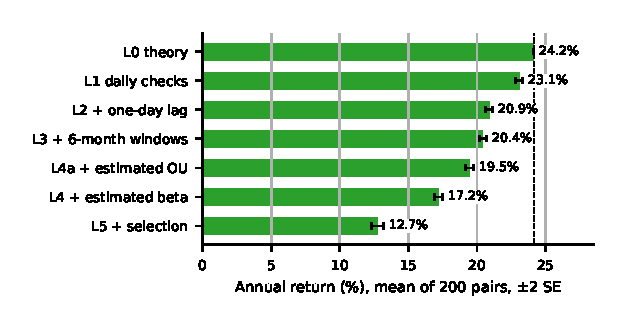
\includegraphics[width=\linewidth]{fig_e4_synthetic_report}
\column{0.38\textwidth}
  \footnotesize\raggedright
  A made-up pair that follows the OU model exactly, 200 runs through the real pipeline:
  \begin{itemize}\setlength{\itemsep}{2pt}
    \item theory \textbf{24.2\%} a year
    \item pipeline \textbf{12.7\%}
    \item biggest loss: picking the pair, $-4.5$ points
  \end{itemize}
\end{columns}
\pairTakeaway{The selection test finds this genuine pair in only 74\% of windows.}
\end{frame}
           % 13 Results E4          M1  1:15
% Slide 14 | Results | M4 (Vismay Shanbhag) | 1:15 | E5, the headline backtest on US stocks
\begin{frame}{E5: no rule is significant on US stocks, yet the signal is real}
\framesubtitle{Slide 14 \textbullet\ Results \textbullet\ M4 \textbullet\ 1:15}
\vspace{-2pt}
\begin{columns}[T,onlytextwidth]
\column{0.45\textwidth}
  \scriptsize\setlength{\tabcolsep}{4pt}
  \begin{tabular}{@{}lrr@{}}
    \toprule
    Rule & Return \%/yr & Sharpe (SE) \\
    \midrule
    S0 Distance & $-0.09$ & $-0.05$ (0.25) \\
    S1 z-score  & 0.33 & \textbf{0.19} (0.25) \\
    S2 s-score  & 0.10 & 0.06 (0.25) \\
    S3 Bertram  & 0.12 & 0.06 (0.25) \\
    \bottomrule
  \end{tabular}\\[5pt]
  \footnotesize\raggedright
  \begin{itemize}\setlength{\itemsep}{2pt}
    \item S1 earns about 44 bp per trade before costs
    \item but 28--45\% of trades never close ($\approx -3\%$ each)
  \end{itemize}
\column{0.50\textwidth}
  \centering
  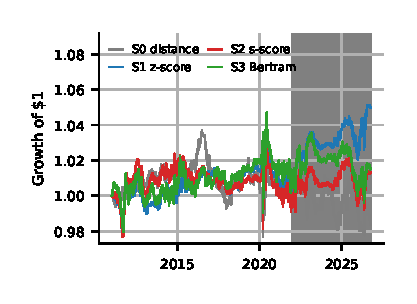
\includegraphics[width=\linewidth]{fig_e5_cumulative_report}
\end{columns}
\pairTakeaway{Only about 8 of 196 candidate pairs pass the test, no more than chance.}
\end{frame}
            % 14 Results E5          M4  1:15
% Slide 15 | Results | M5 (Saatwik Tiwari) | 1:30 | E8: India
\begin{frame}{E8: India repeats the US result}
\framesubtitle{Slide 15 \textbullet\ Results \textbullet\ M5 \textbullet\ 1:30}
\vspace{-2pt}
\begin{columns}[T,onlytextwidth]
\column{0.50\textwidth}
  \footnotesize\setlength{\tabcolsep}{4pt}
  \begin{tabular}{@{}lrrr@{}}
    \toprule
    Rule & Return \%/yr & Sharpe (SE) & Test block \\
    \midrule
    S0 Distance & 0.43 & 0.16 (0.27) & $-0.09$ \\
    S1 z-score  & 0.41 & \textbf{0.38} (0.27) & 0.28 \\
    S2 s-score  & 0.37 & 0.32 (0.27) & 0.56 \\
    S3 Bertram  & 0.43 & 0.32 (0.27) & 0.82 \\
    \bottomrule
  \end{tabular}\\[2pt]
  {\scriptsize 26 NSE stocks, 2013--2026, 15 bp; test block = 2022--2026}
\column{0.46\textwidth}
  \small\raggedright
  \begin{itemize}\setlength{\itemsep}{3pt}
    \item all four rules gain slightly, none significantly
    \item only about 3 of 55 pairs pass per window
  \end{itemize}
\end{columns}
\pairTakeaway{Same story as the US: too few genuine pairs for a significant return.}
\end{frame}
                  % 15 Results E8          M5  1:30
% Slide 16 | Results | M2 (Nitin Sureshkumar) | 1:15 | E9: do the selected pairs stay pairs?
\begin{frame}{E9: selected pairs do not stay pairs}
\framesubtitle{Slide 16 \textbullet\ Results \textbullet\ M2 \textbullet\ 1:15}
\vspace{-2pt}
\begin{columns}[T,onlytextwidth]
\column{0.48\textwidth}
  \small\raggedright
  The same ADF test, on the six months after selection (259 US pairs):\\[6pt]
  \centering
  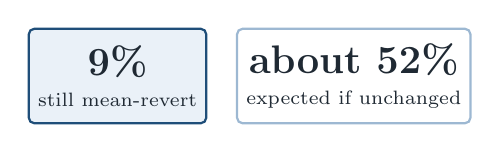
\begin{tikzpicture}
    \node[draw=deckAccent, fill=deckSoft, thick, rounded corners=2pt, minimum width=2.1cm, minimum height=1.2cm, align=center, text=deckInk] at (0,0) {\Large\bfseries 9\%\\[-1pt]\scriptsize still mean-revert};
    \node[draw=deckRule, fill=white, thick, rounded corners=2pt, minimum width=2.1cm, minimum height=1.2cm, align=center, text=deckInk] at (3.0,0) {\Large\bfseries about 52\%\\[-1pt]\scriptsize expected if unchanged};
  \end{tikzpicture}
\column{0.48\textwidth}
  \small\raggedright
  \begin{itemize}\setlength{\itemsep}{3pt}
    \item the 52\% is generous, since fitted speeds are too fast (E1); a fairer figure is lower but well above 9\%
  \end{itemize}
\end{columns}
\pairTakeaway{Selected pairs mostly do not keep their mean reversion: selection picks lucky pairs.}
\end{frame}
            % 16 Results E9          M2  1:15
% Slide 17 | Conclusion | M1 (Lakshya Satya) | 0:45 | conclusions
\begin{frame}{Conclusions}
\framesubtitle{Slide 17 \textbullet\ Conclusion \textbullet\ M1 \textbullet\ 0:45}
\vspace{-2pt}
\normalsize
\begin{columns}[T,onlytextwidth]
\column{0.31\textwidth}
  \textbf{\color{deckAccent}1\ \ Detect}
  \begin{itemize}\setlength{\itemsep}{2pt}
    \item one year finds only fast mean reversion
    \item most selected pairs soon stop mean-reverting
  \end{itemize}
\column{0.31\textwidth}
  \textbf{\color{deckAccent}2\ \ Model}
  \begin{itemize}\setlength{\itemsep}{2pt}
    \item the OU model and Bertram's formula are correct
    \item but $\kappa$ is hard to estimate
  \end{itemize}
\column{0.31\textwidth}
  \textbf{\color{deckAccent}3\ \ Trade}
  \begin{itemize}\setlength{\itemsep}{2pt}
    \item the signal is real before costs
    \item after costs no rule is significant
  \end{itemize}
\end{columns}
\pairTakeaway{The weak link is \textbf{pair selection}, not the trading rules.}
\end{frame}
            % 17 Conclusion          M1  0:45

\end{document}
